\chapter{Evaluation}
\label{cha:evaluation}
 
\section{Location data characteristics for Berlin area}

\subsection{General overview}

Movement triggered data from mobile devices are spanned across the Germany as shown on \autoref{fig:ger_points}. 
\begin{figure}[!ht]
	\centering
	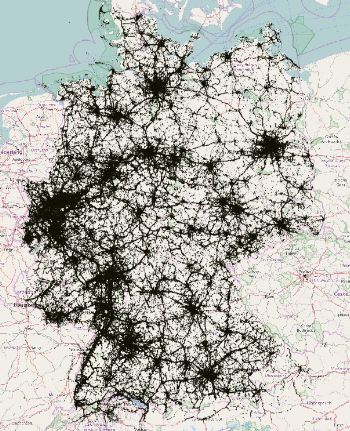
\includegraphics[width=0.3\textwidth]{images/points_germany.png}\\
	\caption{Visualisation of data points location in the geographical map of Germany}
	\label{fig:ger_points}
\end{figure}
\FloatBarrier
It points out, that most of the detected movements from one point to another are mostly gathered on the highways and inside the cities. 
\\
\begin{figure}[!ht]
	\centering
	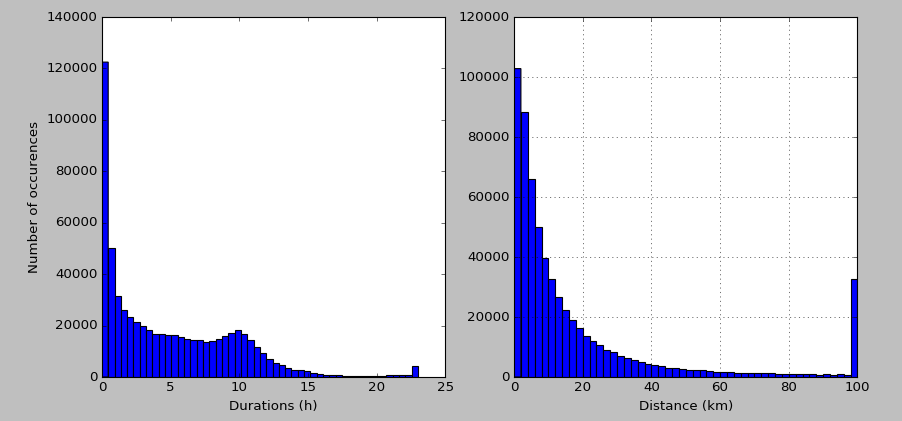
\includegraphics[width=0.9\textwidth]{images/germany_stats.png}\\
	\caption{Histograms of durations and distances between consecutive points under and cumulatively over 100 km for the area of Germany}
	\label{fig:ger_stats}
\end{figure}
\FloatBarrier
The given data batch has been gathered in the interval of 24h starting from 3am in the morning German time. It consists of over 675000 data points, belonging to 47300 unique mobile devices. \autoref{fig:ger_stats} shows, that for unique mobile devices, the durations between consecutive points in time are most frequent within 30 minutes and most of the data is in the interval 1-10h. Regarding distances, consecutive points are most frequent below 2 km and most data is in the interval 0-10km. Big chunk of distances is also over 100km.     
\\
\begin{figure}[!ht]
	\centering
	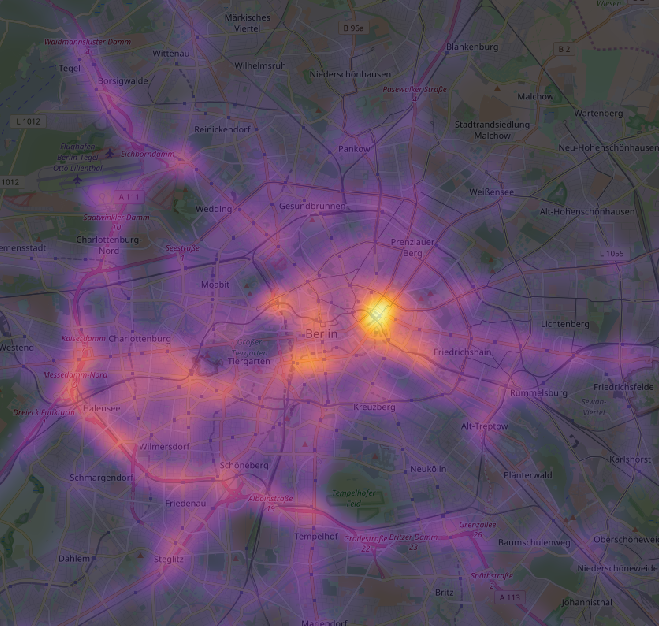
\includegraphics[width=0.9\textwidth]{images/points_berlin_heatmap.png}\\
	\caption{Heatmap of data point densities within the area of Berlin}
	\label{fig:ber_heat}
\end{figure}
\FloatBarrier
\autoref{fig:ber_heat} shows the heatmap of data points for Berlin area. We can see that most of the movements detected are on major train/tram/metro stations, highways and major living areas. 

\subsection{Data analysis}
\label{cha:dataanaly}

Statistics performed using tool written in Python (https://github.com/mrow4a/macroscopic-movements-algorithm-prototypes) shows, that for users at least once visiting Berlin, had in average 17 points gathered because of their movements in the period of 24h, harmonic mean of 4 points and maximum 100 of points.
\\
\begin{figure}[!ht]
	\centering
	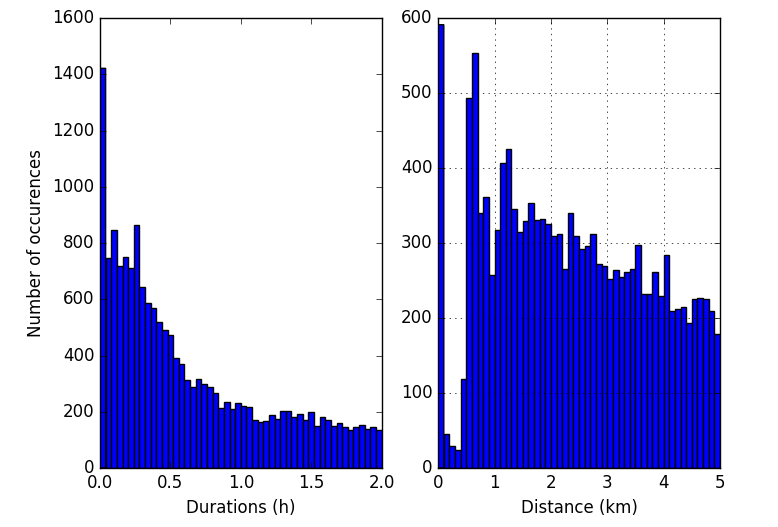
\includegraphics[width=0.6\textwidth]{images/berlin_stats_intro.png}\\
	\caption{Histograms of durations and distances between consecutive points under 5 km and under durations of 2h for the area of Berlin}
	\label{fig:ber_stats}
\end{figure}
\FloatBarrier
Furthermore, majority of durations between points is within interval of 30 minutes. For distances between points, there is significant "jump" at 500-1000m and 1100-1500m, which might mean that at these intervals, continuous points been gathered, and distances over that values might be discontinuous (ref. \autoref{fig:movement_update} ). It is due to the fact that these distance intervals are most frequent and that might suggest that this is an average "update" distance for the moving mobile devices, as described in \autoref{cha:introduction_methodo}. Less frequent values might suggest that updates were obtained with lower accuracy (e.g. by presence inside the building, metro line or simply mobile device lag in obtaining its location) and are result of discontinuity between consecutive updates.
\begin{figure}[!ht]
	\centering
	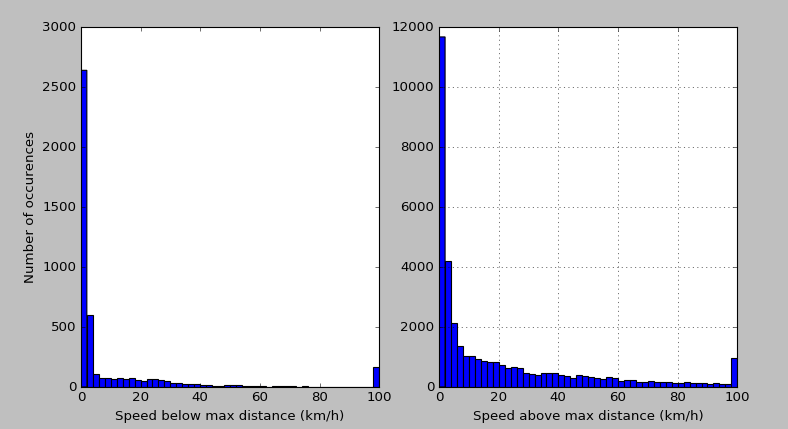
\includegraphics[width=0.6\textwidth]{images/berlin_speeds_distances.png}\\
	\caption{Histogram of speed between points with corresponding distance above or below 1.5 km}
	\label{fig:ber_sp_dis}
\end{figure}
\FloatBarrier
\autoref{fig:ber_sp_dis} shows that considering the registered distances within range of 1500m, the wast majority of points are between 0-2 km/h, and also significant interval at 2-6 km/h. The rest of the values is sparse distributed in interval 6-100+ km/h. In case of registered point above range of 1500m, we observe that indeed most frequent occurrence is at interval of 0-4 km/h, however most are sparse distributed above 4 km/h, with most points being in interval of 4-20 km/h. 

\section{Pre-filtering of anomalies}
\label{cha:prefilter}
\autoref{fig:ber_stats} shows that there is a fraction of points which duration or distance rapidly changed, thus resulting in very high speeds between the points. Furthermore, due to the methodology of obtaining points (movement triggered), there are some minimum distances and durations at which points can be collected, and values not matching stop or travel expectation according to gathered statistics, have to be filtered. Thus, the following predicates for filtered values have been set:
\begin{description}
	\item[Jumps] Points with speed over 83 m/s [300 km/h]
	\item[Duplicates] Points with distance below 100m and at the same time duration below 10s
\end{description}

\section{Evaluation of stop detection algorithms}

\begin{figure}[!ht]
	\centering
	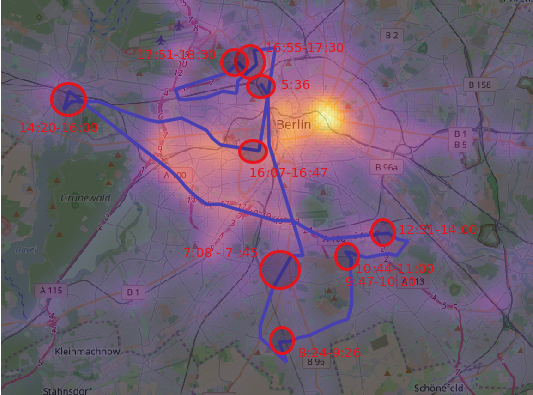
\includegraphics[width=0.6\textwidth]{images/reco_example_1a.png}\\
	\caption{ Visualization of distances, speed and mobility indexes for example from \autoref{fig:reco_example_1b} with identified stop candidates }
	\label{fig:reco_example_1a}
\end{figure} 
\begin{figure}[!ht]
	\centering
	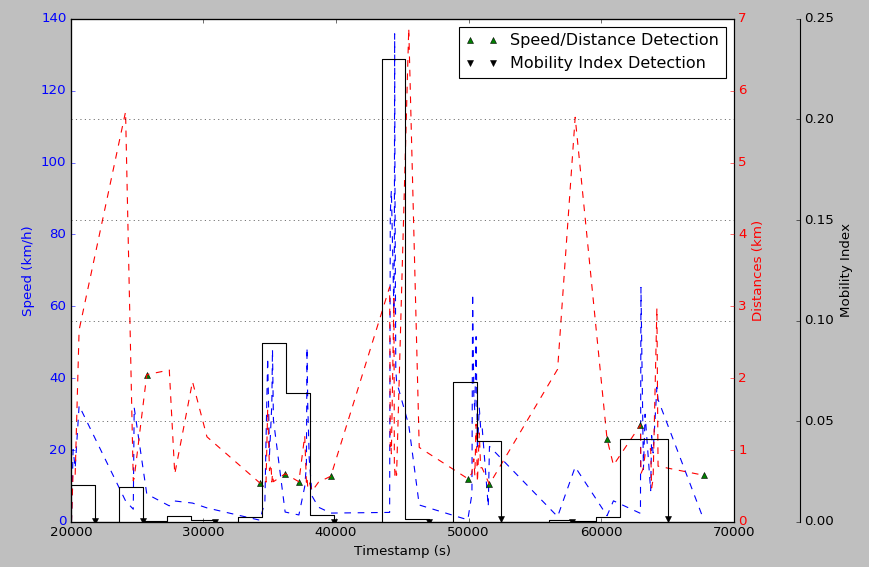
\includegraphics[width=0.6\textwidth]{images/reco_example_1b.png}\\
	\caption{ Movement example for one user in the period of 24h, with recorded locations due to the movement and annotated timestamps for detected stop candidates }
	\label{fig:reco_example_1b}
\end{figure}
\FloatBarrier

\subsection{Mobility Index approach with varying time window}

TODO

\subsection{Mobility Index approach with varying threshold}

TODO

\subsection{Human Mobility approach for long/short distances}

TODO

\subsection{Effectiveness of approaches}

TODO

\section{Clustering algorithm}

In this section we will describe how we evaluated our dbscan algorithm and the choice of the \textit{epsilon} and \textit{minimum points per cluster} parameter.

\subsection{DBSCAN}

We visualised our results in QGIS, a powerful graph visualisation tool. Running the dbscan with different parameters resulted in different cluster sizes and number of clusters. We started off with the target area of Berlin. The \textit{epsilon} parameter (radius of the cluster) was chosen by looking at the graininess (accuracy) of our given data set. The accuracy between points was 110 meters, this distance is refered to as \textit{accuracy distance}.
We took Alexanderplatz in Berlin as an example cluster (a popular train stop area in Berlin). We interpret one cluster as being one stop point of interest, and for this application want Alexanderplatz to be represented as one cluster. Setting the \textit{epsilon} parameter to the \textit{accuracy distance},  110 meters, gave us good looking clusters whilst higher value of the parameter resulted in clusters being unnaturally large and distance below the \textit{accuracy distance} resulted in only single-point clusters (points are stacked at the same location). Note that the \textit{minPts}, minimum points per cluster, parameter is not taken into \textit{consideration} here (it is set arbitary and only determines the number of clusters, while we here are interested in the \textit{size} of the clusters). See figures below.

\begin{figure}[!ht]
	\centering
	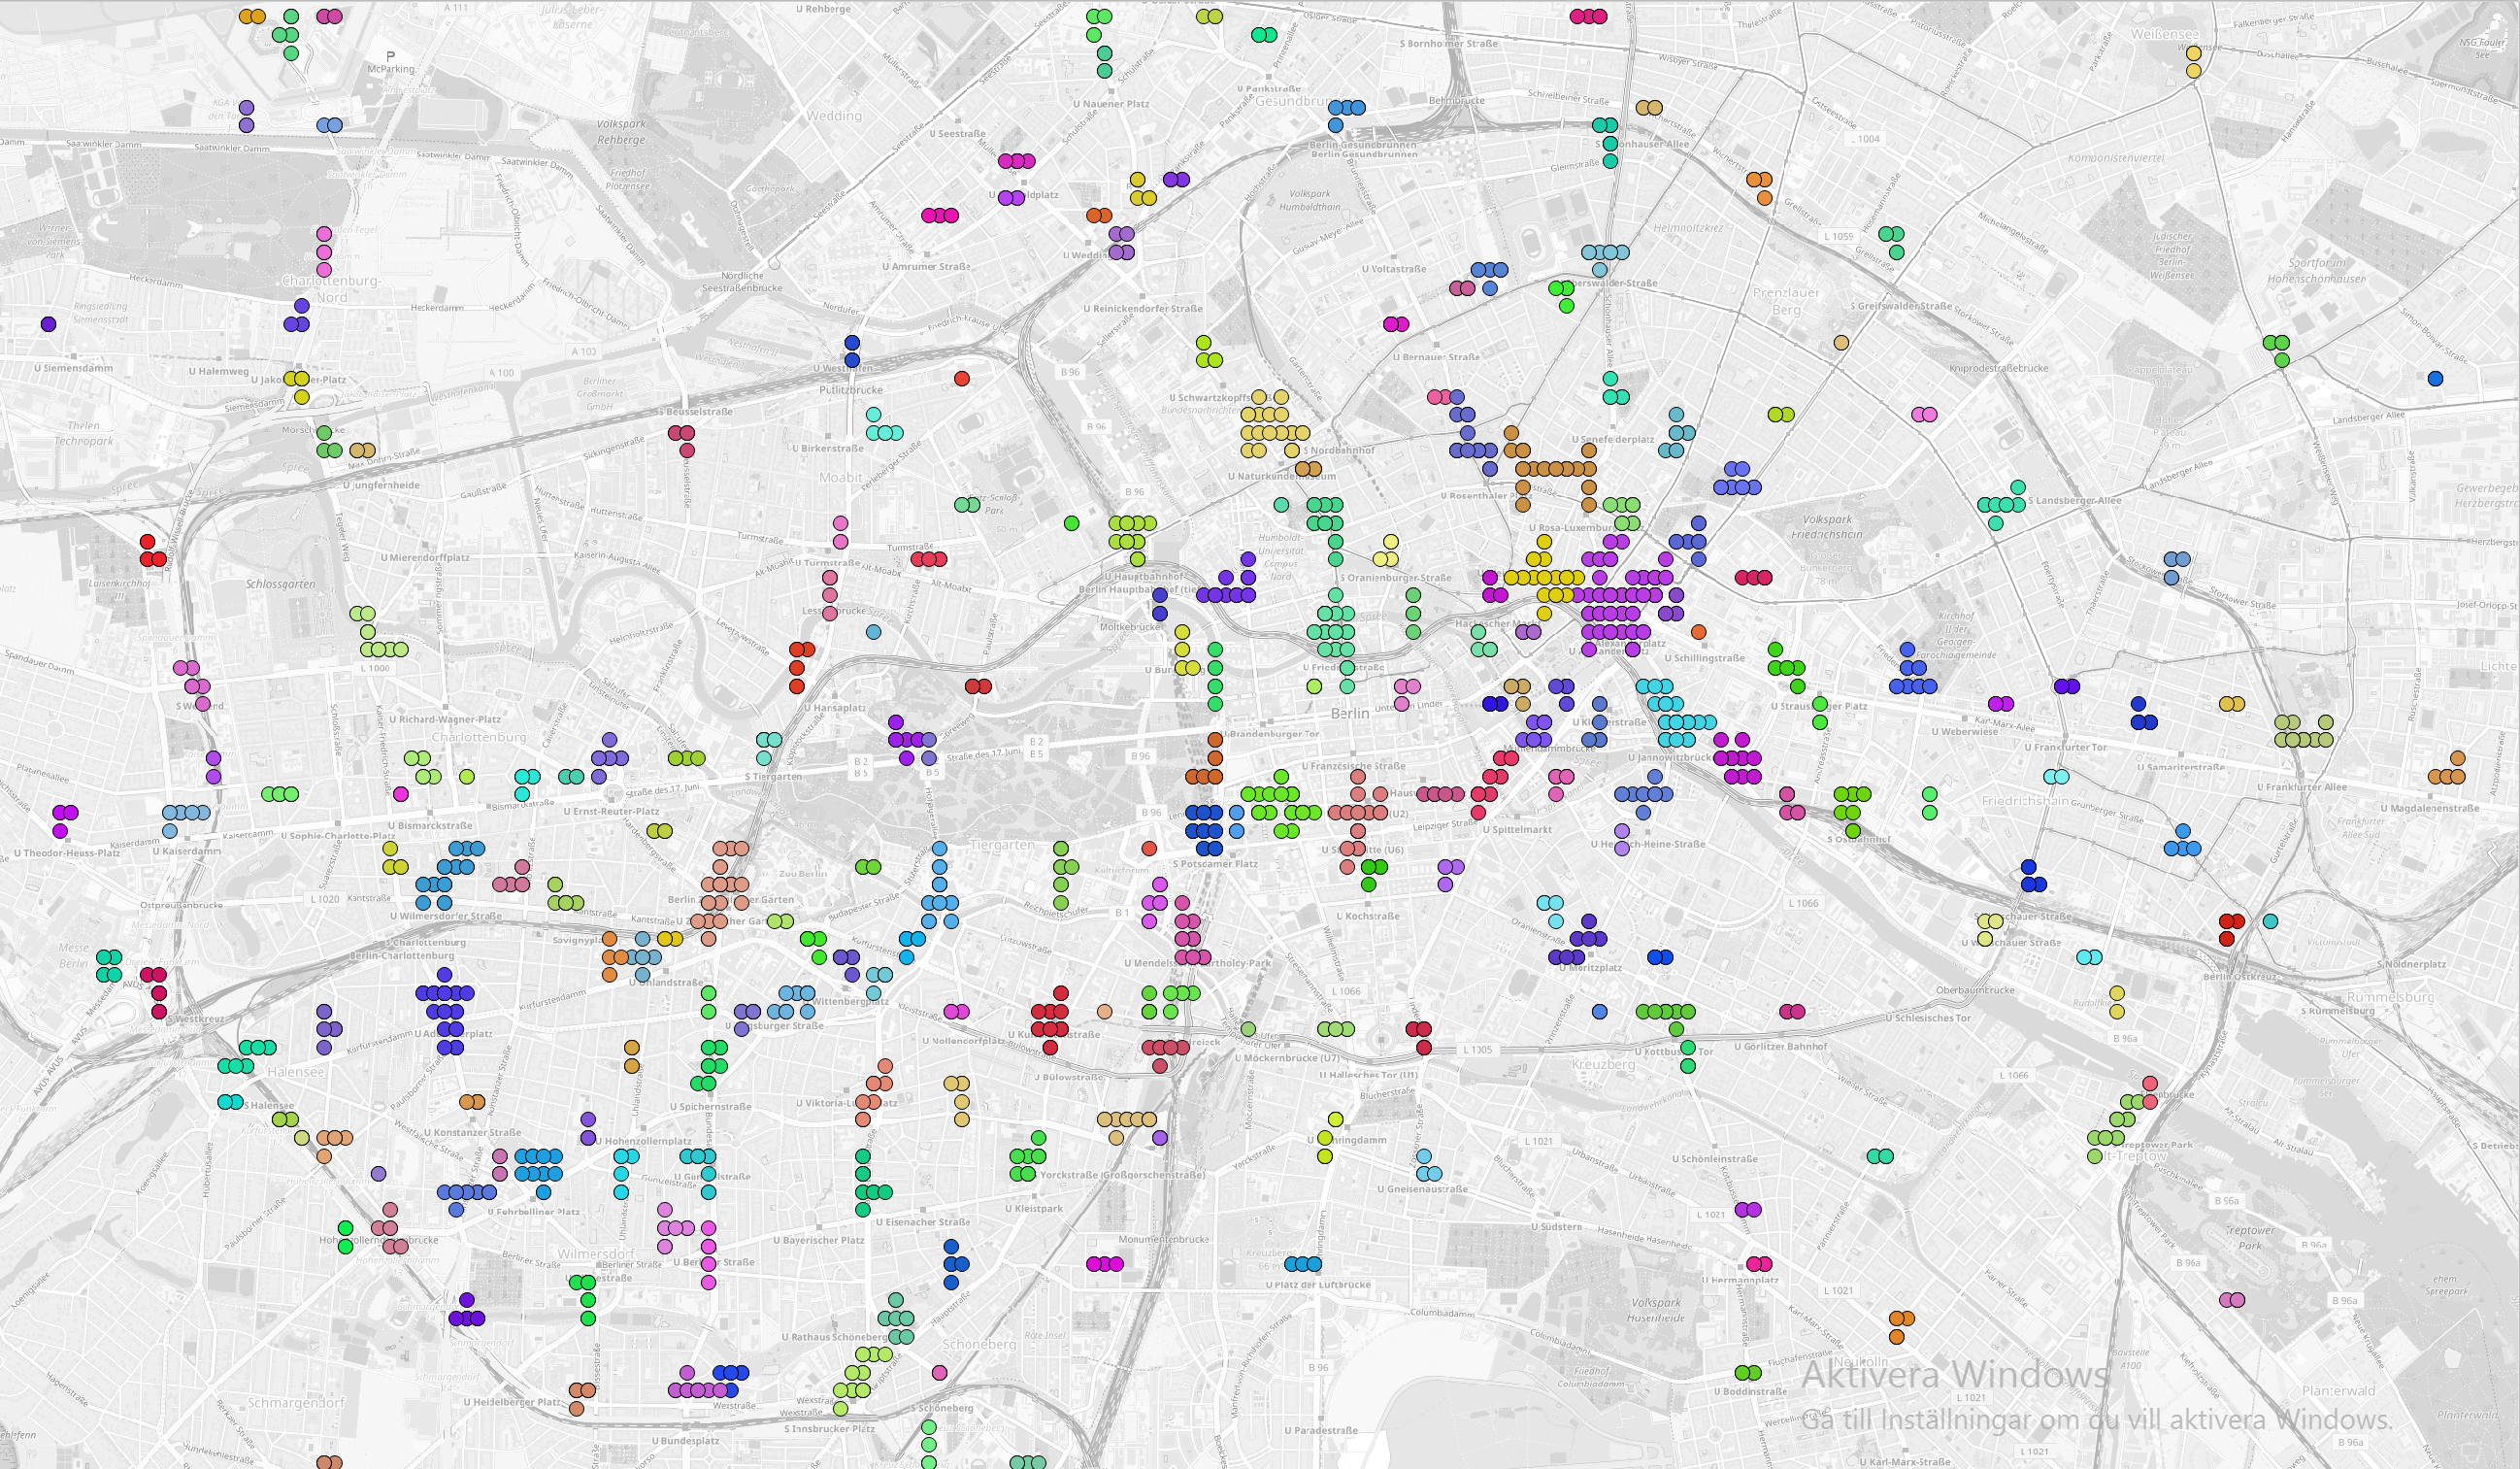
\includegraphics[width=1\textwidth]{images/0,001_5_gray.png}\\
	\caption{ Clusters with good parameters \textit{epsilon} = 110 meter, \textit{minPts} = 5. Alexanderplatz (pink) has 85 data points in it.  }
	\label{fig:0.001_5_gray}
\end{figure}

\begin{figure}[!ht]
	\centering
	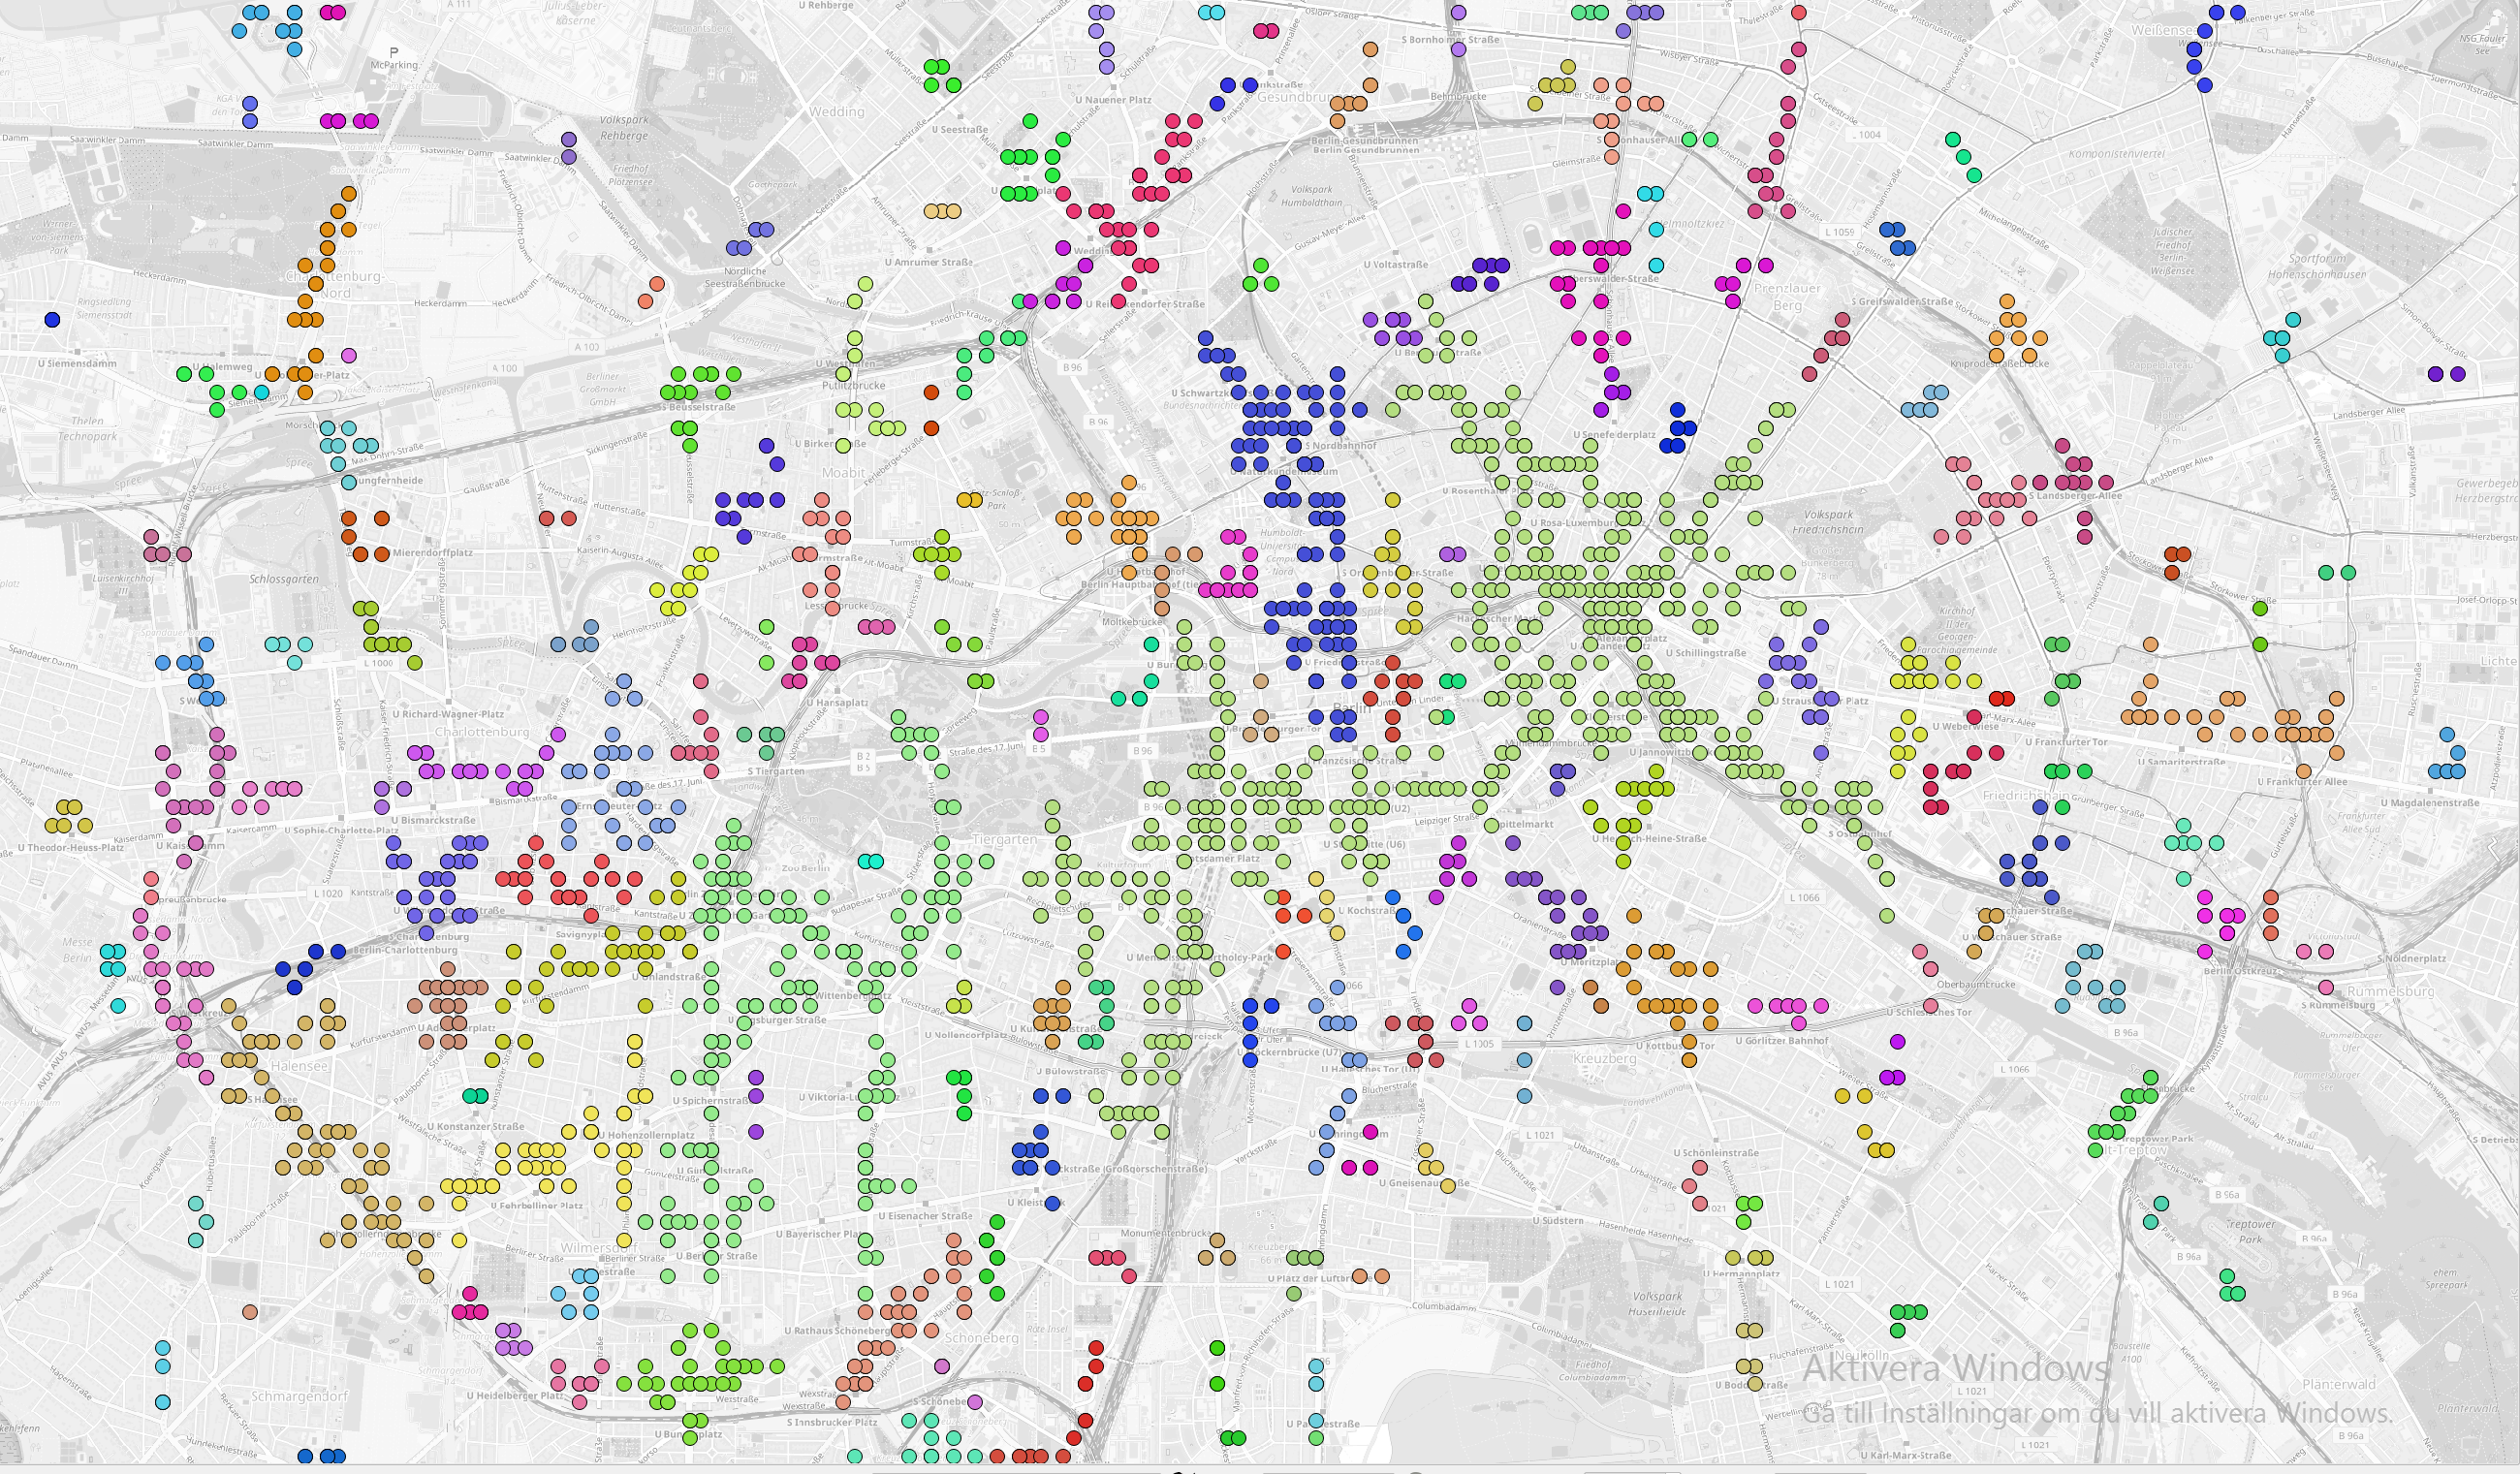
\includegraphics[width=1\textwidth]{images/0,002_5_gray.png}\\
	\caption{ Example of a clusters with bad parameters, here \textit{epsilon} = 220 meter is too large, \textit{minPts} = 5. "Alexanderplatz" (light green) has 748 data points in it and stretches over the whole centre (Mitte) of Berlin. }
	\label{fig:002_5_gray}
\end{figure}